\section{Introcution}

In this lab, we will get used to the WiFi system and accomplish the sampling and measuring of WiFi signal strength through programming in Android on smartphone. Based on the skeleton codes, we will compile them and run on a actual Android phone. We will collect the signal strength of the WiFi AP nearby and analyze them. Furthermore, we will implement the function of locating user's position.

\section{Environment Setup}

The environment of this experiment is listed as follows. I could not run Android Studio on my computer and used Intellij IDEA as an alternative.

\begin{itemize}
  \item Development Envrionment OS: macOS 11.2
  \item IDE: Intellij IDEA Ultimate 2020.2
  \item Android SDK 26
\end{itemize}

Note that a few classes (such as \texttt{android.support.v4.app.ActivityCompat}) used in \texttt{MainActivity.java} are deprecated. Following the hints of Intellij IDEA, we port them to the current environment (changed to \texttt{androidx.core.app.ActivityCompat}). Furthermore, we also changed the layout of the \texttt{activity\_main.xml} so that the current SDK could compile it.


\section{WiFi Signal Strength}

The skeleton has implemented the following function:
\begin{enumerate}
  \item User click the \texttt{SCAN} button. \texttt{MainActivity.java} will respond to the click event by creating a \texttt{SuperWifi.java} class.
  \item {SuperWifi.java} obtain the SSID groups by \texttt{mWiFiManager.startScan()} function.
  \item {SuperWifi.java} will select the user expected APs and record their signal strength 10 times.
  \item {SuperWifi.java} write the results into an output file. The scanning ends.
  \item {MainActivity.java} notifies users by showing a message in the TextView area of the application.
\end{enumerate}

In order to port to SDK 26, we rewrite the user interface \texttt{activity\_main.xml}. To help with debugging, we allow users to specify which APs should be measured in the user interface, so that the APs are no longer hard-encoded into the code. We also change some codes in \texttt{SuperWifi.java} in order to fit our new design.

We test the basic functions on Android Emulator, the results are shown in Figure \ref{fig:test1} and \ref{fig:test2}. Note that the emulator only simulates a Wifi AP called \texttt{AndroidWifi}, so we get constant results.



\begin{figure}[t]
  \centering
  \begin{minipage}[t]{0.48\linewidth}
  \centering
    \caption{Emulation Demo}
    \label{fig:test1}
    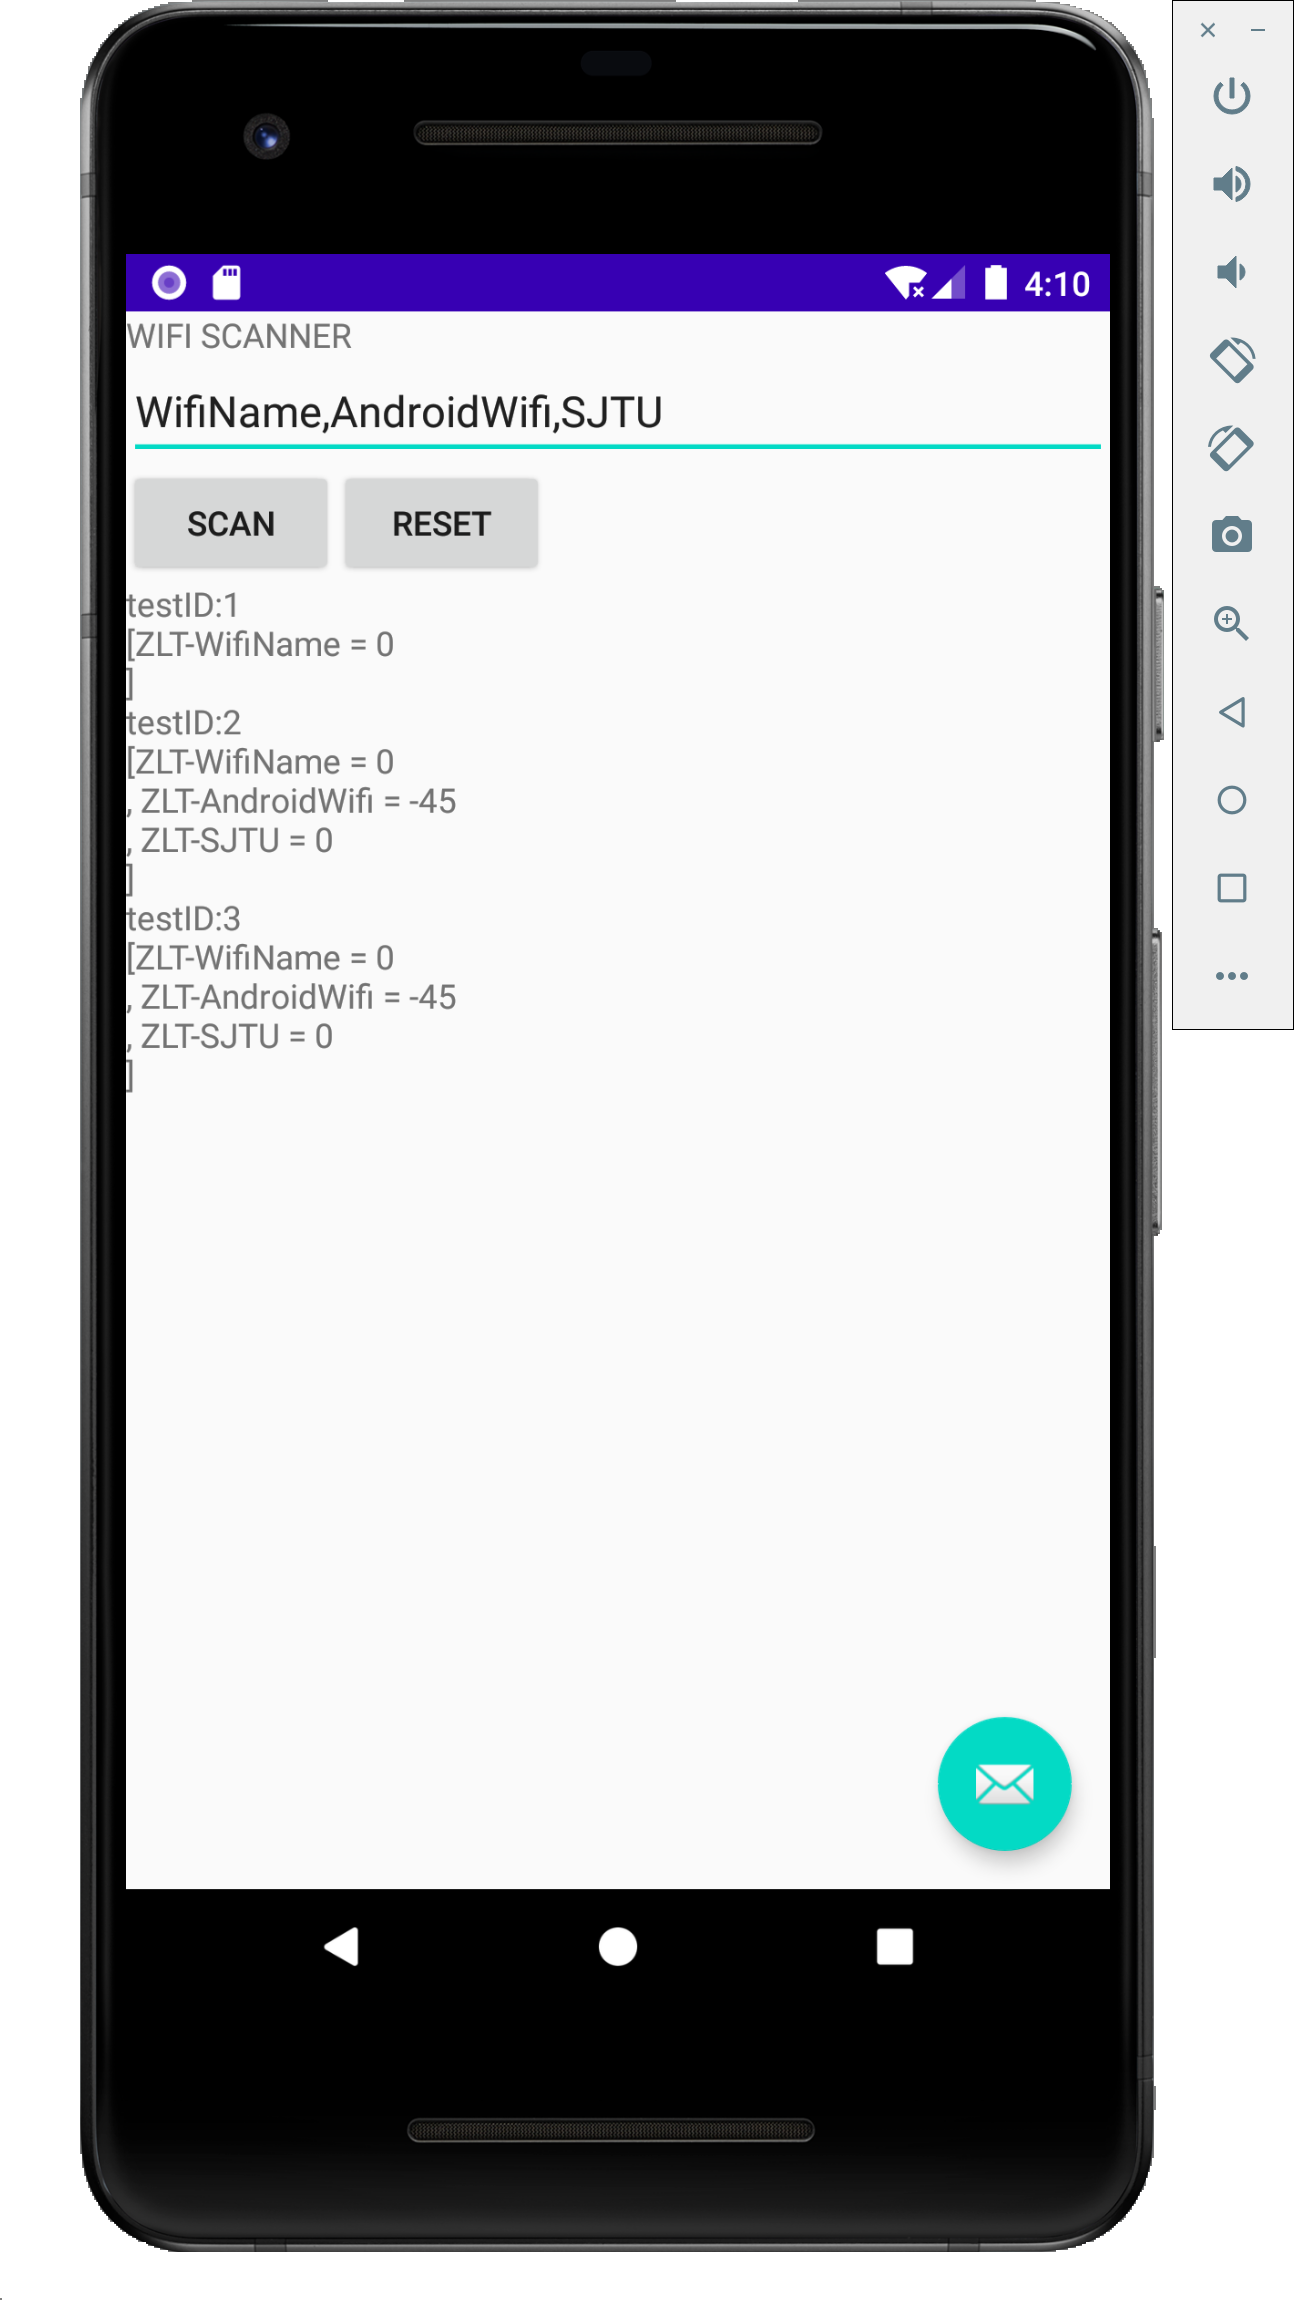
\includegraphics[width=0.8\columnwidth]{img/test1.png} 
    \end{minipage}
    \begin{minipage}[t]{0.48\linewidth}
    \centering
      \caption{Output Result}
      \label{fig:test2}
      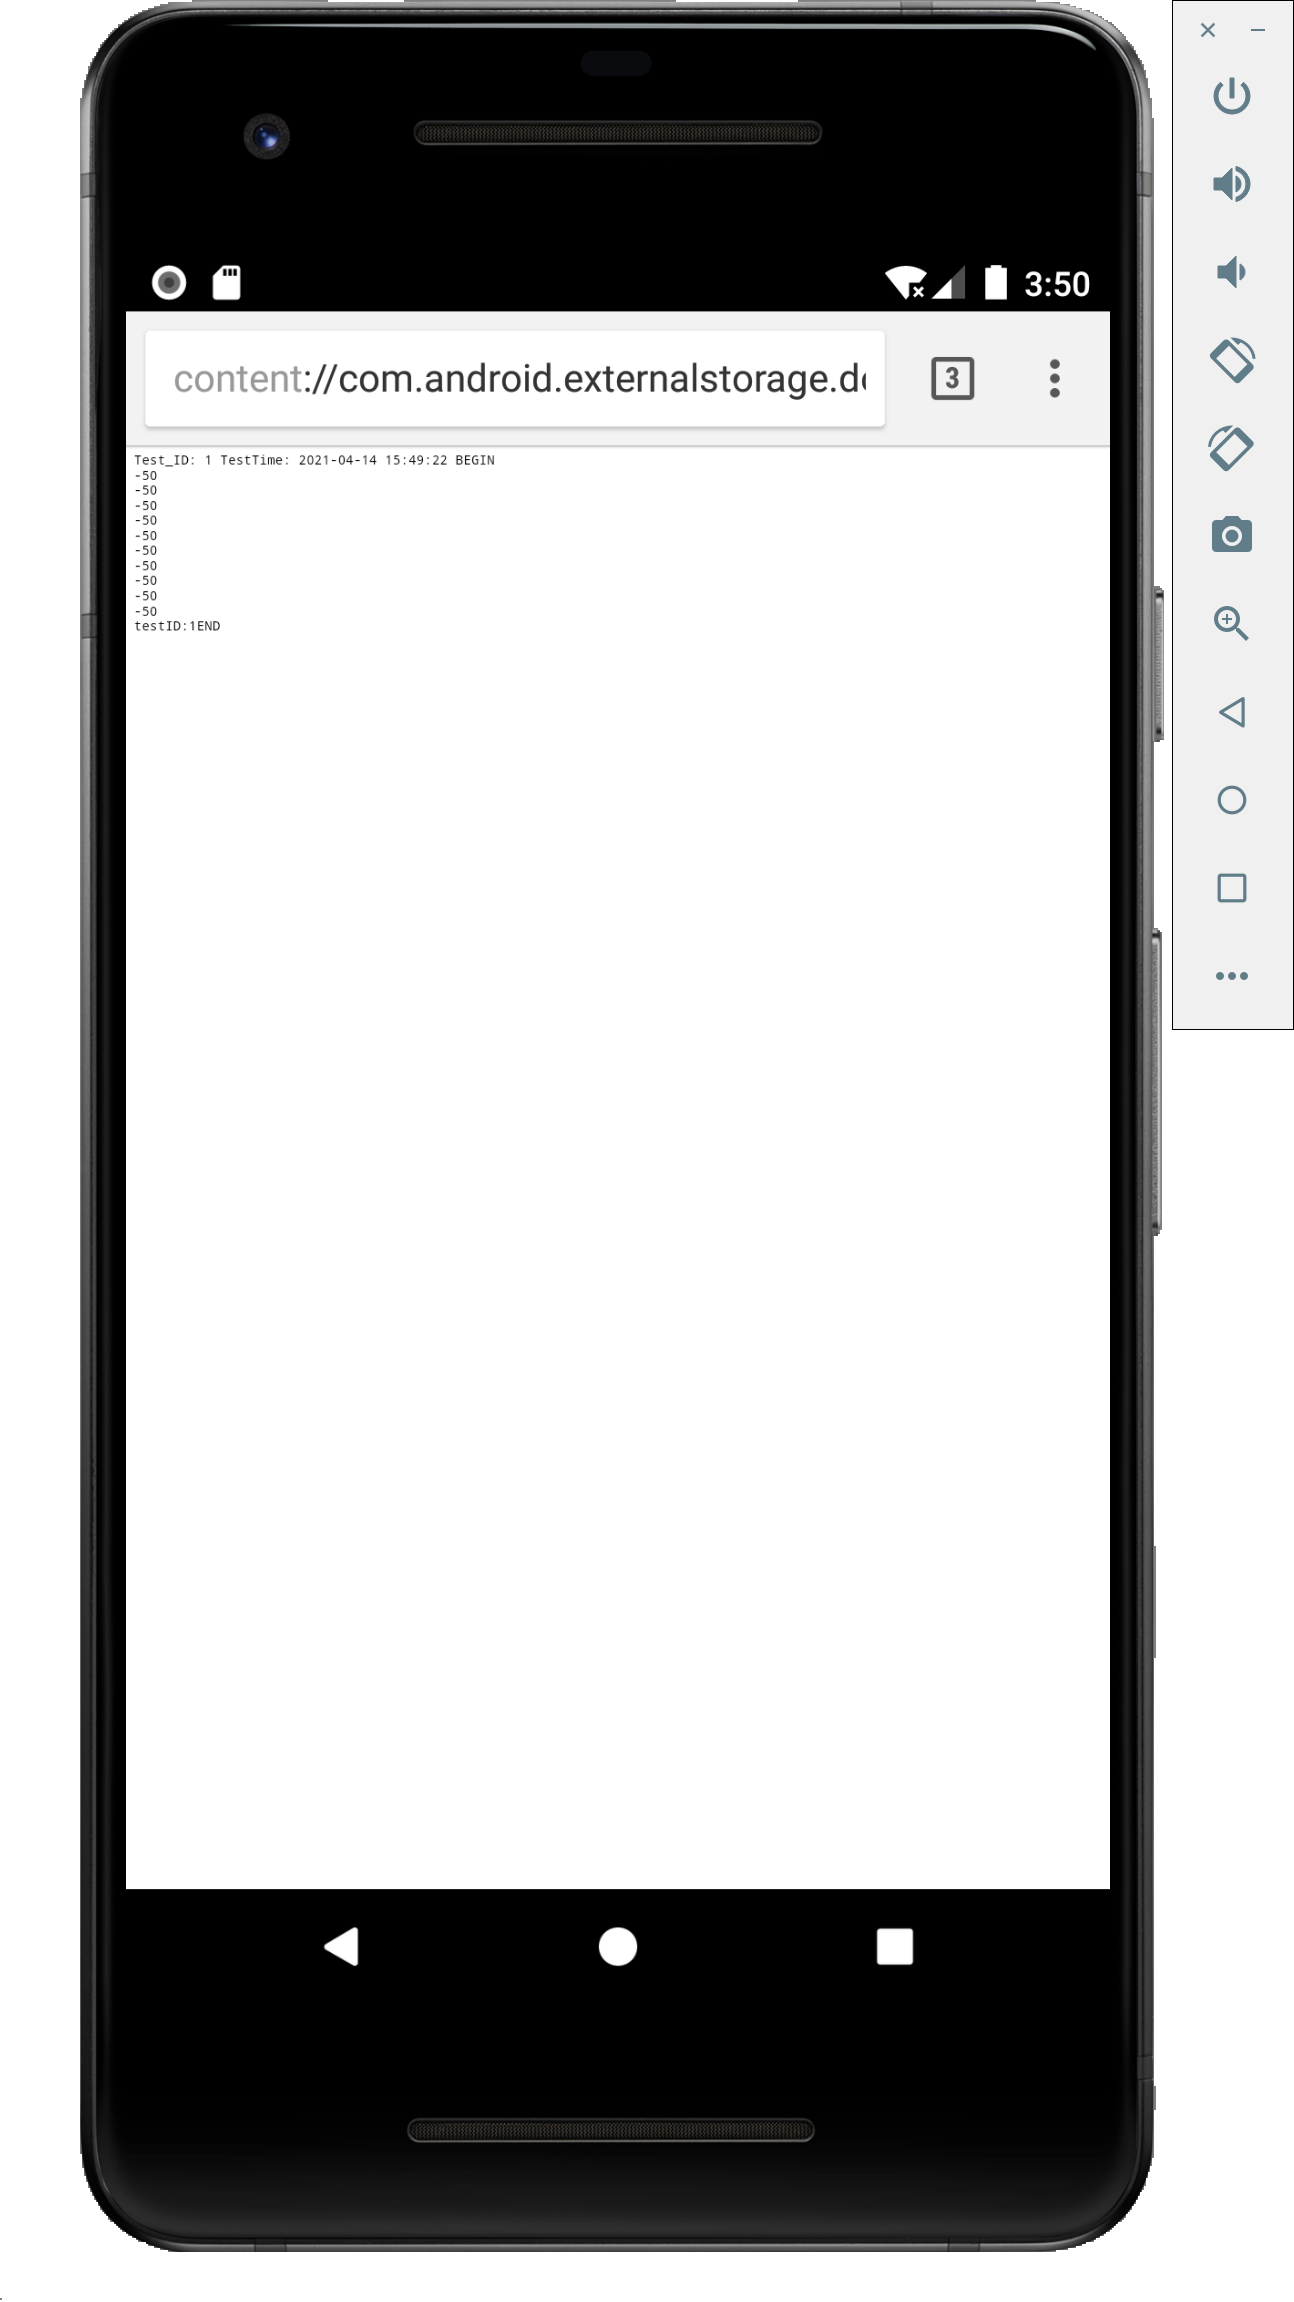
\includegraphics[width=0.8\columnwidth]{img/test2.png} 
    \end{minipage}
\end{figure}


\section{Questions}
\begin{enumerate}
  \item Why is necessary to record all the measured value rather than only the average value?
  
  From the experiment we know that the WiFi strength we test at a particular moment is very unstable. However, user usually expects a stable value. Therefore, it is important that our application can identify the outliers that are extremely off the average. By taking the record of all measured value, we can identify the irregular measurement out and evaluate the confidence of the result of a scanning.

  \item Besides the WiFi signal strength, what other information of the Routers can be got in the test?
  
  We may refer to the system API document to identify what attributes we can get. See Figure \ref{fig:attr}. We list a few as follows:
  \begin{itemize}
    \item \texttt{SSID}: The network name.
    \item \texttt{BSSID}: The address of the access point.
    \item \texttt{level}: The detected signal level in dBm, also known as the RSSI.
    \item \texttt{capabilities}: Describes the authentication, key management, and encryption schemes supported by the access point.
    \item \texttt{frequency}: The primary 20 MHz frequency (in MHz) of the channel over which the client is communicating with the access point.
  \end{itemize}

  \begin{figure}[hb]
    \begin{center}
    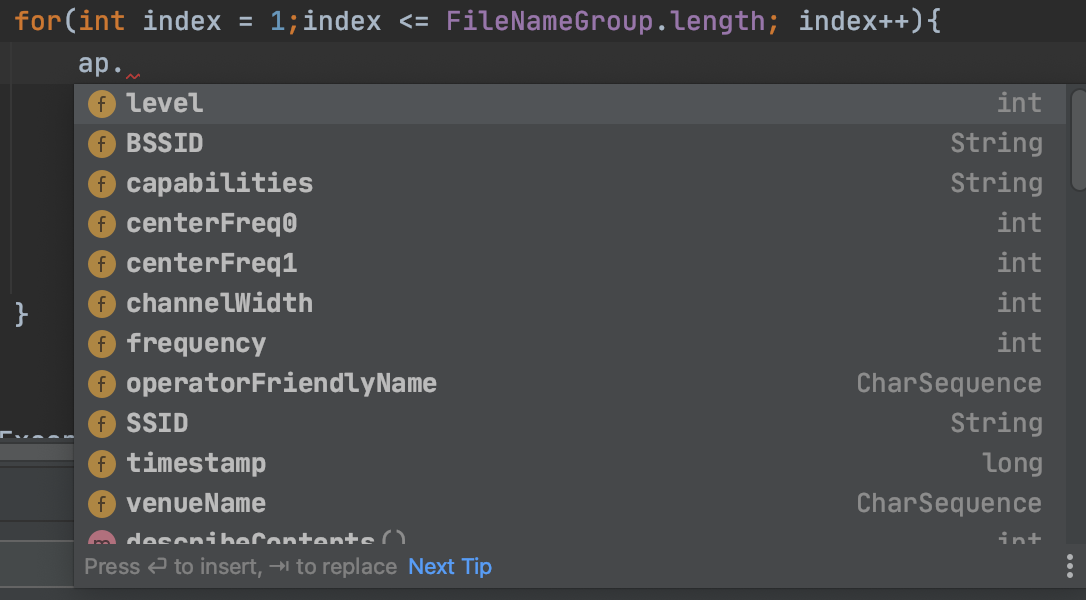
\includegraphics[width=12cm]{img/attr.png}
    \caption{AP attributes}
    \label{fig:attr}
    \end{center}
  \end{figure}

  \item Why does the scanning need to be operated in thread ``scanThread''?
  
  ScanThread takes a long time because we need to repeatedly record the WiFi signal strength. If we don't let the scanning be a separate thread from the main process, every time user launches a scan command, the main process will be blocked, which will degrade user's experience.
  

\end{enumerate}